
LoRaWAN je otevřený standard, který řeší problematiku přenosu dat z koncových
zařízení skrze brány na internetové servery. Koncová zařízení v síti LoRaWAN
komunikují pomocí modulace LoRa nebo FSK.

LoRaWAN mimo jiné specifikuje:

\begin{itemize}
    \item Postup připojování nových koncových zařízení
    \item Volbu optimálních přenosových rychlostí
    \item Zabezpečení přenášených dat --- šifrování a kontrolu integrity
    \item Případné potvrzování odeslaných/přijatých dat
    \item Identifikaci přenášených dat aplikačními porty
\end{itemize}

Rozdíl mezi standardy LoRa a LoRaWAN je podobný např. rozdílu mezi WiFi a HTTP; 
jsou to technologie řešící odlišné vrstvy komunikace, které mohou, ale nemusí
být používány společně.

V této kapitole je popsán standard LoRaWAN ve verzi 1.0.4, protože to je verze,
kterou implementuje použitá knihovna LoRaMac-node poslední vydané (a v této
práci použité) verzi v4.5.1.
Nejnovější vydanou verzí LoRaWAN v době psaní této práce je však verze 1.1.0,
která mj. rozšiřuje seznam klíčů použitých při komunikaci.

% https://lora-alliance.org/resource-hub/lorawanr-specification-v11


Podrobnosti rádiových komunikacím, zejména dostupné frekvence a omezení 
vysílacího času se liší mezi regiony, zde vycházím z evropských podmínek.
Tyto na regionu závislé parametry jsou uvedeny v dokumentu LoRaWAN Regional
Parameters v1.1rA.

% https://lora-alliance.org/resource-hub/lorawanr-regional-parameters-v11ra

% https://lora-alliance.org/resource-hub/what-lorawanr

Stejně jako např. mnoho domácností provozuje své WiFi sítě, které všechny 
odpovídají stejnému standardu (popř. různým verzím stejného standardu) a 
technicky je tedy možné, pokud to provozovatel povolí, aby zařízení přecházela
z jedné sítě do jiné, i standard LoRaWAN předpokládá a umožňuje
provoz LoRaWAN sítí různými operátory, kteří mohou rozhodnout, kterým koncovým
zařízením povolí připojit se.

\section{Architektura sítě LoRaWAN}

    \label{subsubsec:LoRaWAN_architecture}

    LoRaWAN má hvězdicovou architekturu, ilustrovanou na obrázku 
    \ref{fig:LoRaWAN_architecture}. Figurují v ní následující typy zařízení:

    \begin{itemize}
        \item Koncová zařízení (End nodes)
        \item Brány (Concentrator/Gateway)
        \item Síťové servery (Network Server)
        \item Aplikační servery (Application Server)
        \item Připojovací servery (Join Server) --- na obrázku neuvedeno
    \end{itemize}

    Síťové, připojovací a aplikační servery mohou být různá vzájemně 
    komunikující fyzická zařízení. 
    V případě sítě TTN, použité v této práci, jsou však všechny tři 
    funkcionality implementovány v rámci síťového serveru.

    \begin{figure}[h]
        \begin{centering}
            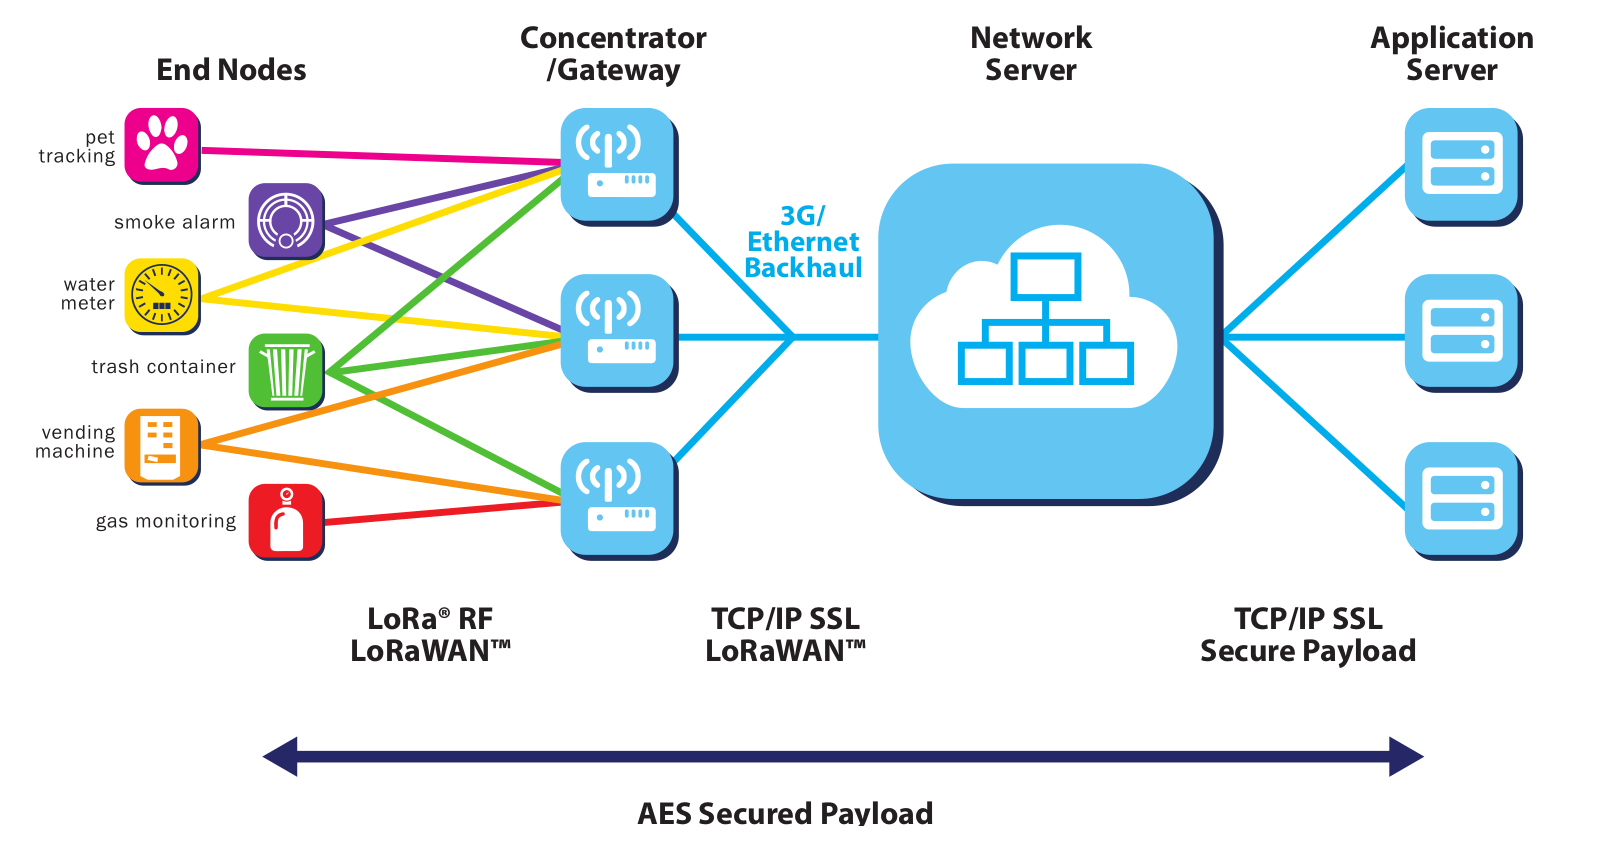
\includegraphics[width=1\textwidth]{Figures/lorawan}
            \caption{Architektura sítě LoRaWAN}
            \label{fig:LoRaWAN_architecture}
        \end{centering}
    \end{figure}

    Před tím než koncové zařízení může komunikovat v LoRaWAN síti, musí být
    aktivováno (tj. nakonfigurováno). 
    Více k tomuto tématu v \ref{subsubsec:LoRaWAN_activation}.

    Koncová zařízení pak vysílají svá data pomocí LoRa či FSK modulace. 
    Ta jsou zachycena jednou či více branami, které je zašlou pomocí běžných 
    internetových komunikačních technologií (IP, mobilní sítě ap.) na LoRaWAN 
    síťový server. Ten zprávy zkontroluje, odstraní ty které jsou poškozené či 
    duplikované, a zašle data na příslušný aplikační server provozovatele daného 
    koncového zařízení. 

    Předpokládá se tedy, že jeden operátor, provozující síťový server (servery)
    a brány poskytuje kapacitu své sítě různým zákazníkům, kteří mají svá koncová
    zařízení a mohou mít své aplikační servery. 
    Je však samozřejmě možné, aby operátor provozoval
    a poskytoval i aplikační servery.

    Komunikace mezi koncovým zařízením a bránou může být obousměrná,
    viz \ref{subsubsec:LoRaWAN_Classes}.

    V LoRaWAN síti se očekává pouze komunikace mezi koncovým zařízením a aplikačním
    serverem skrze bránu a síťový server,
    nikoli mezi zařízeními navzájem. Taková komunikace LoRa protokolem mezi
    koncovými zařízeními však technicky možná \emph{je}.

    % Co je to aplikace v kontextu LoRaWAN?

\section{Třídy koncových zařízení}
    \label{subsubsec:LoRaWAN_Classes}

    Třída zařízení určuje, jak často zařízení naslouchá datům zaslaným z brány.
    Čím častěji zařízení naslouchá příchozím datům, tím více energie 
    spotřebovává, zároveň je ale o to rychleji schopno na přijatá data reagovat.

    LoRaWAN definuje následující třídy:    
    \begin{description}
        \item [Třída A] Zařízení naslouchá naslouchá pouze ve dvou krátkých 
            časových úsecích poté, co odeslalo data.
        \item [Třída B] Zařízení naslouchá stejně často jako zařízení třídy A,
            a navíc v pravidelných intervalech synchronizovaných se
            signálem vysílaným bránou.
        \item [Třída C] Zařízení naslouchá nepřetržitě, kromě doby kdy samo vysílá.
    \end{description}

    Každé zařízení připojené do LoRaWAN musí implementovat alespoň třídu A.

    Volba třídy zařízení je tedy kompromisem mezi spotřebou energie a rychlostí
    odezvy na zaslaná data. 
    Vlastnosti třídy A se nejvíce hodí pro senzory zasílající malá množství dat
    v dlouhých časových intervalech, napájené z baterií.
    Zařízení s dostatkem energie a vyššími požadavky na rychlost
    odezvy na zaslaná data pak mohou implementovat třídu B či C.

    Pro implementaci dané třídy je nutné pouze příslušné softwarové vybavení
    koncového zařízení; hardwarovými požadavky se třídy navzájem neliší.

    Cílem této práce je vytvořit zařízení třídy A; ostatním třídám se proto
    dále nevěnuji.

\section{Přístup k médiu, rychlosti a frekvence rádiové komunikace}

    Podrobnosti rádiových komunikacím, zejména dostupné frekvence a omezení 
    vysílacího času se liší mezi regiony, zde vycházím z podmínek v České 
    Republice. Tyto na regionu závislé parametry jsou uvedeny v dokumentu 
    LoRaWAN Regional Parameters v1.1rA.
    % https://lora-alliance.org/resource-hub/lorawanr-regional-parameters-v11ra

    Koncová zařízení mohou vysílat v jakémkoli okamžiku, musí však
    splnit následující podmínky:

    \begin{itemize}
        \item Každá vysílaná zpráva musí být vyslána na odlišném kanálu 
            (tj. frekvenci) než předcházející
        \item Zařízení musí respektovat omezení (zejm. vysílacího času) dané 
            platnou legislativou
    \end{itemize}    
 
    Kromě LoRa komunikace mohou koncová zařízení při dobrých přenosových
    podmínkách použít LoRaWAN standardem podporovanou FSK modulaci. Ta má sice
    nižší dosah, ale cca 
    pětinásobně vyšší přenosovou rychlost než nejrychlejší LoRa komunikace. 
    Tabulka \ref{tab:LoRaWAN_datarates} uvádí přenosové rychlosti v LoRaWAN 
    sítích pro Evropu.

    \begin{table}[h]
        \begin{center}
            \caption{Datové rychlosti používané v LoRaWAN síti v Evropě}
            \label{tab:LoRaWAN_datarates}    
            \begin{tabular}{p{0.25\textwidth}<{\centering}
                    |p{0.25\textwidth}|p{0.25\textwidth}}
                \hline 
                \textbf{Číselné označení datové rychlosti (DR)} 
                & \textbf{Konfigurace vysílání} (Typ modulace, SF hodnota, 
                    šířka pásma) 
                &  \textbf{Bitová rychlost (bps)}\\
                \hline 
                DR0 & LoRa SF12/125 kHz & 250\\
                DR1 & LoRa SF11/125 kHz & 440\\
                DR2 & LoRa SF10/125 kHz & 980\\
                DR3 & LoRa SF9/125 kHz & 1760\\
                DR4 & LoRa SF8/125 kHz & 3125\\
                DR5 & LoRa SF7/125 kHz & 5470\\
                DR6 & LoRa SF7/250 kHz & 11000\\
                DR7 & FSK: 50 kbps & 50000\\
                \hline
                DR8 až DR14 & \multicolumn{2}{c}
                    {Rezervováno pro budoucí užití}\\
                \hline
                DR15 & \multicolumn{2}{c}{Definováno standardem LoRaWAN} \\
                % footnote here!
                \hline
            \end{tabular}        
        \end{center}
    \end{table}

    LoRaWAN vyžaduje, aby každé zařízení bylo schopno komunikovat alespoň
    na třech kanálech uvedených v tabulce \ref{tab:LoRaWAN_reqChannels}.

    \begin{table}[h]
        \begin{center}
            \caption{Kanály, na kterých musí být každé připojené zařízení schopno komunikovat}
            \label{tab:LoRaWAN_reqChannels}
            \begin{tabular}{c|c|c} % column alignments
                    \textbf{Šířka pásma (kHz)} 
                    & \textbf{Frekvence kanálu (MHz)} 
                    & \textbf{Datová rychlost} \\
                \hline
                125 & 868.1 & DR0 - DR5 \\
                125 & 868.3 & DR0 - DR5 \\
                125 & 868.5 & DR0 - DR5 \\
                \hline
            \end{tabular}
        \end{center}
    \end{table}

    Pro optimalizaci rádiového provozu v síti a úsporu energie spotřebované 
    pro vysílání je v LoRaWAN použit ADR mechanismus.
    Ten nastavuje jednotlivým zařízením optimální rychlosti komunikace.

    Protože jedním z hlavních legislativních omezení provozu v ISM pásmech je 
    vysílací čas, zajišťuje ADR mechanismus aby zařízení komunikovala co možná
    nejvyšší rychlostí, a tedy po co nejkratší dobu.
    
    Díky tomu že se rádiové provozy LoRa komunikace různých rychlostí navzájem
    neruší, je možné, aby různě vzdálená zařízení užívající různé rychlosti
    komunikovala současně.
    Jediným omezením je pak schopnost brány naslouchat více komunikacím 
    najednou.

\section{Připojení do sítě}\label{sec:act}
    \label{subsubsec:LoRaWAN_activation}

    Zařízení komunikující v LoRaWAN síti musí být tzv. aktivováno. 
    Aktivace slouží k získání parametrů potřebných pro komunikaci v síti, 
    zejména pak klíčů k šifrování a zajištění integrity.

    Tyto parametry jsou:

    \begin{description}
        \item [DevAddr] 32 bitová adresa, jež slouží k identifikaci koncového
            zařízení v rámci jedné sítě. Skládá se z:
            \begin{description}
                \item [AddrPrefix] odvozeno z identifikačního čísla sítě
                \item [NwkAddr] přiděleno síťovým serverem
            \end{description}
            poměr délek těchto částí je možno pozměnit dle potřeby
        \item [NwkSKey] 128 bitový AES klíč, unikátní pro každé zařízení,
            sloužící k šifrování MAC příkazů
            % co jsou to MAC příkazy?
        \item [AppSKey] 128 bitový AES klíč, sloužící k šifrování komunikace 
            mezi koncovým zařízením a aplikačním serverem.
    \end{description}

    Existují dva způsoby aktivace --- ABP a OTAA.

    \subsection{ABT - Activation by Personalization}
        \label{par:LoRaWAN_ABP}

        Spočívá ve fixním nastavení parametrů komunikace při výrobě zařízení.
        Ihned po startu je tak zařízení schopno vysílat a přijímat data,
        neevýhodou je však vazba zařízení na síť jednoho konkrétního operátora.
        Tento způsob je snadnější na implementaci, ale obecně není doporučován,
        a v této práci není použit.

    \subsection{OTAA - Over the Air Activation}
        \label{par:LoRaWAN_OTAA}

        Při použití OTAA nejsou klíče pro komunikaci uloženy v zařízení před
        připojením do sítě, ale jsou získány při procesu připojování. Výhodou
        tohoto způsobu je možnost přecházet mezi sítěmi různých operátorů, a
        také možnost změny použitých klíčů zopakováním procedury aktivace,
        např. v případě že klíče byly ztraceny/objeveny nežádoucí třetí stranou.

        Pro OTAA aktivaci musí koncové zařízení mít k dispozici následující 
        informace:

        \begin{description}
            \item [DevEUI]
                je 64 bitový identifikátor, jedinečný pro toto zařízení v rámci
                všech LoRaWAN sítí. Tento identifikátor by měla mít i zařízení
                používající aktivaci ABP.
            \item [JoinEUI]
                je 64 bitový identifikátor, identifikující použitý Join server
            \item [AppKey]
                128 bitový klíč, který je znám pouze tomuto zařízení a jeho
                uživateli, resp. aplikačnímu serveru. Operátor sítě jej nezná.
        \end{description}

        Proces OTAA aktivace se skládá ze dvou fází:

        \begin{enumerate}
            \item Koncové zařízení odešle Join-Request žádost, obsahující 
                \texttt{JoinEUI}, \texttt{DevEUI} a \texttt{DevNonce}. 
                Tato žádost je nešifrovaná, ale je podepsaná \texttt{AppKey} 
                klíčem a ochráněné \texttt{DevNonce} hodnotou (popsána níže)
                --- není tedy možné ji podvrhnout.
            \item Pokud síťový server žádost obdrží a rozhodne se zařízení 
                přijmout, odpoví mu zprávou Join-Accept, ve které mu poskytne
                \texttt{DevAddr}, \texttt{JoinNonce} a některé další informace,
                které slouží pro odvození klíčů potřebných pro komunikaci.
                \texttt{JoinNonce} slouží mj. pro ochranu před falešnými 
                síťovými servery.
        \end{enumerate}

        Pole \texttt{DevNonce} je číslo uložené v koncovém zařízení, které je 
        při vůbec první Join-Request žádosti zařízením odeslané nastaveno na 0,
        a pro každou další odeslanou Join-Request zprávu zvýšeno.
        % A nebo Join-Server???
        Síťový server si pamatuje poslední hodnotu \texttt{DevNonce} se kterou
        se dané zařízení připojilo, a v případě že obdrží Join-Request požadavek
        s hodnotou \texttt{DevNonce} nižší než poslední, pak jej zahodí.
        Toto zajišťuje ochranu v případě, že by útočník zachytil jednu z
        dříve odeslaných Join-Request žádostí, a chtěl by se jejím opětovným 
        odesláním připojit, a předstírat tak identitu danoho koncového zařízení
        bez znalostí jeho \texttt{AppKey}.
        Je nutné, aby si zařízení pamatoval poslední použitou hodnotu 
        \texttt{DevNonce} i v případě ztráty napájení atp.

\section{Zprávy posílané v LoRaWAN síti a jejich zabezpečení}

    Data zasílaná mezi koncovým zařízením a síťovým serverem lze rozdělit na tři
    kategorie:

    \begin{description}
        \item [Uživatelská data] jsou data, která síťový server přeposílá na
            příslušný aplikační server (např. data ze senzoru).
        \item [MAC příkazy] jsou příkazy komunikované pouze mezi síťovým 
            serverem a MAC částí koncového zařízení, která se stará o samotnou
            LoRaWAN komunikaci (viz \ref{subsubsec:LoRaWAN_node_arch}). 
            Jsou to například zprávy související s ADR.
        \item [OTAA zprávy] jsou zprávy sloužící k připojení zařízení do sítě
            a vyjednání potřebných parametrů komunikace. Více k tomuto tématu
            v \ref{par:LoRaWAN_OTAA}.
    \end{description}

    Tyto tři kategorie zpráv se liší v zabezpečení --- uživatelská data jsou 
    šifrována klíčem \texttt{AppKey} známým pouze koncovému zařízení a aplikačnímu serveru,
    zatímco MAC příkazy jsou šifrovány \texttt{NwkSKey} klíčem známým koncovému zařízení a 
    síťovému serveru. MAC příkazy mohou být odeslány jak síťovým serverem, tak
    koncovým zařízením --- často se skládají z požadavků a odpovědí.

    V jedné zprávě mohou být jen uživatelská data, jen MAC příkazy nebo obojí 
    dohromady (v tom případě je množství MAC příkazů limitováno).

    \subsection{Integrita datového přenou}

        Tj. jistota, že data nebyla mezi odesílatelem a příjemcem pozměněna,
        je zajištěna mezi koncovým zařízením a síťovým serverem pomocí
        \texttt{MIC} části zasílaných zpráv.
        % 6.1.3
        LoRaWAN protokol tedy zajišťuje šifrování dat mezi koncovým zařízením 
        a aplikačním serverem, nicméně integritu dat zajišťuje pouze mezi
        koncovým zařízením a síťovým serverem --- \textbf{neumožňuje} 
        aplikačnímu serveru zjistit, zda síťový server data nepozměnil.
        V případě potřeby lze však integritu dat mezi koncovým zařízením a aplikačním
        serverem zajistit přidanými mechanismy (podepisování zpráv atp.).

    \subsection{Šifrování datového přenosu}

        Pro šifrování dat v LoRaWAN v1.0.4 jsou použity dva klíče: 
        \texttt{NwkSEncKey} a    \texttt{AppSKey}.

        \texttt{NwkSEncKey} je použit k šifrování MAC příkazů, tj. komunikace 
        mezi koncovým zařízením a síťovým serverem.
        
        \texttt{AppSKey} je použit pro šifrování komunikace mezi koncovým
        zařízením a aplikačním serverem. Síťový server tedy obsah komunikace 
        mezi koncovým zařízením a aplikačním serverem \textbf{nevidí}.        

\section{Architektura aplikace koncového zařízení}
    \label{subsubsec:LoRaWAN_node_arch}

    Na obrázku \ref{fig:LoRaWAN_nodeswarch} je ilustrována architektura zařízení 
    komunikujícího v LoRaWAN síti.

    \begin{figure}[h]
        \begin{centering}
            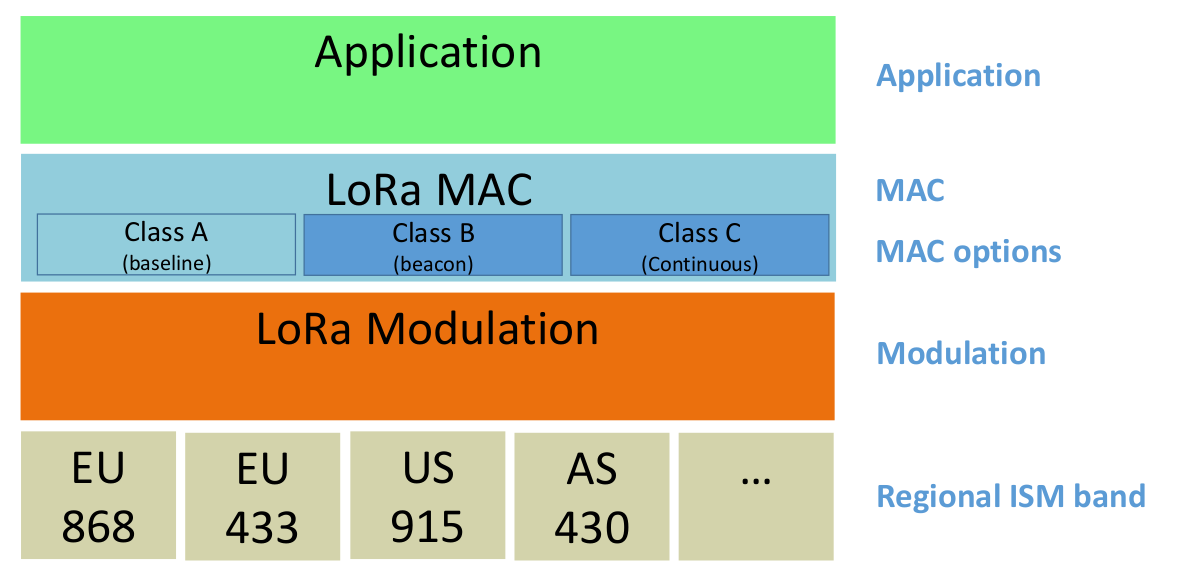
\includegraphics[width=1\textwidth]{Figures/node_architecture}        
            \caption{Architektura aplikace koncového zařízení}
            \label{fig:LoRaWAN_nodeswarch}
        \end{centering}
    \end{figure}

    Aplikaci zařízení, lze, z hlediska LoRaWAN, rozdělit do celkem 4 vrstev:

    \begin{description}
        \item [Aplikace] (Application) --- "uživatelský" program běžící na zařízení. Jeho
            zodpovědností je připravovat data zasílaná na aplikační server,
            popř. reagovat na přijaté požadavky. Pro samotné zasílání dat používá
            API LoRa MAC vrstvy (knihovny).
        \item [LoRa MAC] zodpovídá za vše co souvisí s LoRaWAN standardem. 
            Například aktivace, uchovávání informací souvisejících se spojením,
            zpracování MAC příkazů atp. Pro rádiovou komunikaci používá API
            nižší vrstvy, obvykle rádiového modulu. 
        \item [LoRa Modulation] (LoRa modulace) je obvykle prováděna přislušným
            rádiovým modulem. Jeho zodpovědností je odesílání a příjem LoRa 
            (popř. FSK) paketů. Obsah zpráv, použité frekvence, SF a CR hodnoty
            jsou dány vyšší vrstvou (LoRa MAC).
        \item [Regional ISM band] (regionální ISM pásmo) --- slouží jako médium
            pro bezdrátovou komunikaci. Jeho parametry musí být známy MAC vrstvě.
    \end{description}

